% ==============================================================================================
% 2010-11-05 Preisig, H A       ; NTNU
% 2011-12-15  ditto             ; adapted for PSE 11
%                               ; put all the heading info into the style file
% 2012-01-04  ditto             ; Reference section title fixed -- integrated into style file
%                               ; changed sequence: first bibliography then pse style
%                               ;  pse style redefines reference listing superseding natlib def
%                               ;  and simplified by moving reference style loading into pse.sty
% 2014-09-04  ditto             ; reverted to standard LaTeX fonts
%                               ; issues - measures do not correspond with manual. 
%                               ; There is a cm missing 13.5 textwidth gives 12.5 texwidth ???
% 2015-10-14 Zinser, A          ; adapted to ESCAPE 26
% 2017-11-11 Radl, S            ; adapted to ESCAPE 28
% 2018-10-10 Kiss, A. A.        ; adapted to ESCAPE 29
% 2020-06-25 Türkay, M.         ; adapted to ESCAPE 31
% ==============================================================================================

\documentclass[fleqn,twoside,10pt]{article}

%% bibliography must be before escape styles
\usepackage{natbib}
\bibliographystyle{elsart-harv}

%% Escape/PSE styles
\usepackage{left_eq}   % To get the equation left aligned, this is ugly but required :-)
\usepackage{escape31}  % Stylefile from Escape


%%% >>>>>>>>>>>>>>> use your own GRAPHICS configuration <<<<<<<<<<<<<<<<<<<<<<<
\usepackage{pstricks, pst-plot}	% pstricks
\usepackage{graphicx} % enables import of various formats
\usepackage{wrapfig}  % enables floating wrapped figures
\usepackage[figuresright]{rotating}


%% math packages
\usepackage{amsmath}
\usepackage{amssymb}

%% >>>>>>>>>>>>>>>> user definitions BIBLIOGRAPHY & DEFS <<<<<<<<<<<<<<<<<<<<<<<<


%% personal styles and definitions
%\usepackage{mystyle}
%\def\mydefs{defs}
\usepackage[english]{babel}
\usepackage{blindtext}


% ================================================================================
\title{Type the title of your paper}
%
 \author[a]{Anne Firstauthor}
 \author[b]{Tim B. Secondauthor }
 \author[a,b,*]{James Q. Thirdauthor}
 \affil[a]{First affiliation, Address, City and Postcode, Country}
 \affil[b]{Second affiliation, Address, City and Postcode, Country}
 \email{emailOfTheCorrespondingAuthor@organization.countryCode}
 
 \HeaderTitle{Type the title of your paper}
 \HeaderAuthor{A. Firstauthor et al.}

% ==================================== title ====================================

\begin{document}

\maketitle             % make title page with abstract and keywords
\thispagestyle{empty}  % first page has a different format

% ================================================================================

\begin{abstract}
  \textbf{IMPORTANT}: for the EXACT instructions how to write the paper, please refer to the MS Word template for the paper! 
  
  \textbf{IMPORTANT}: The manuscript must have six pages (including references), not more and not less.
  
  \blindtext
\end{abstract}
\Keywords{add three to five keywords here, separated with a comma}

% ==================================== body  =====================================

\section{Section title}

This is a section

\subsection{Sub-section}

Equations come as normal, the included style file for the left equation notation of Elsevier is automatically included. So for example
\begin{equation}
  A = B + C
\end{equation}
or an aligned equations
\begin{align}
  \dot{x} &= A \, x + B \, u \\
  y &= C \, x
\end{align}
But also the starred versions work:
\begin{equation*}
  A = B + C
\end{equation*}
or an aligned equations
\begin{align*}
  \dot{x} &= A \, x + B \, u \\
  y &= C \, x
\end{align*}

\blindtext[2]

The subsubsection then appears like:

\subsubsection{Subsubsection}
This gives all numbered titles. \cite{Reference2015}

\paragraph{Paragraph}
\begin{wrapfigure}{r}{0.5\textwidth}
  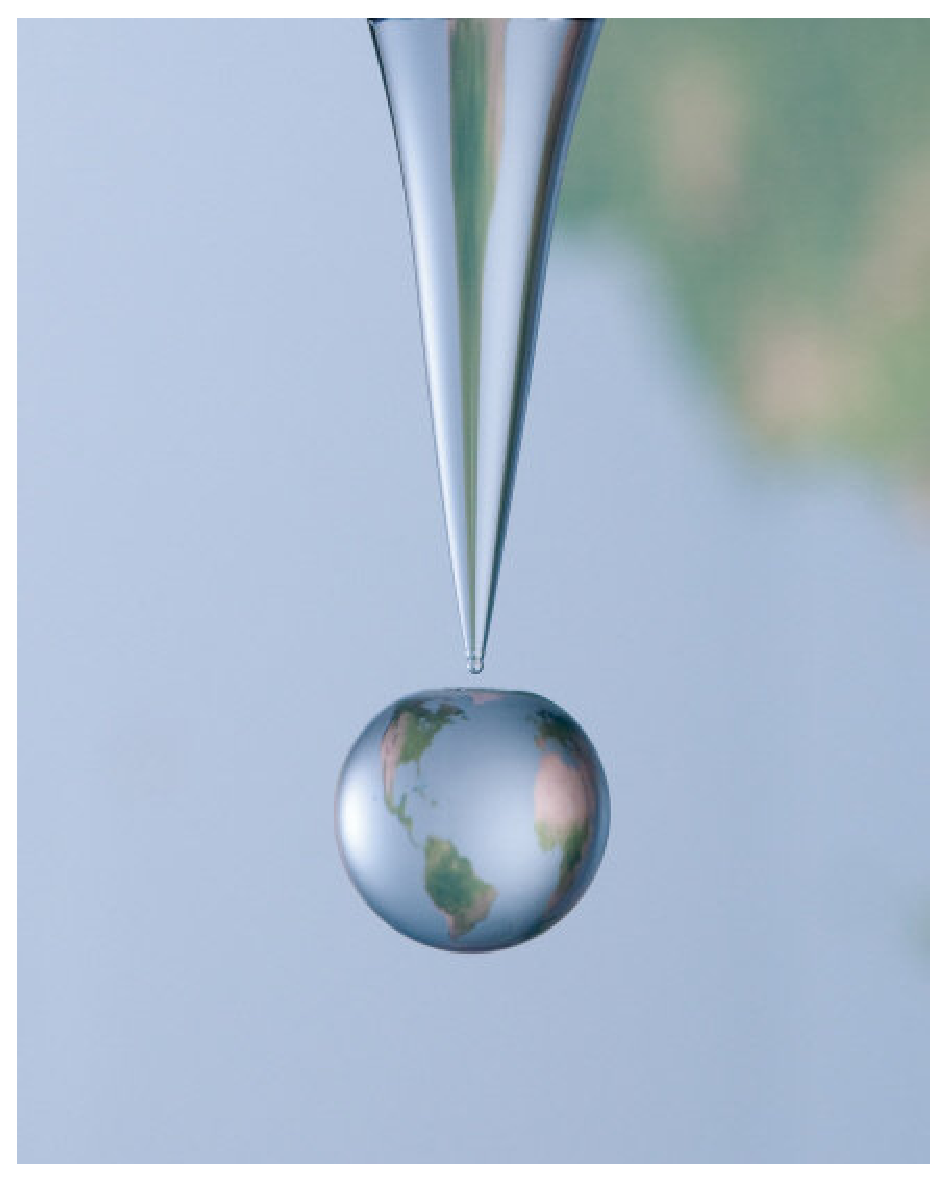
\includegraphics[width=0.5\textwidth]{F_drop.eps}
  \caption{The world in a drop}
  \label{Fig:drop}
\end{wrapfigure}
Figure \ref{Fig:drop} shows the word in a drop -- 

\section{Starred section commands}
The starred section commands, which do not show numbering, are not available.

\section{More}
\blindtext[2]

\section{Much more}
\blindtext[3]


% ================================ references ===================================
%% References 

{\small\bibsep=0pt
\bibliography{example}
}
\end{document}
% ================================== end =========================================